\documentclass[border=10pt]{standalone}
\usepackage[T1]{fontenc}
\usepackage[default]{sourcesanspro}
\usepackage{tikz}
\usepackage{xcolor}
\usetikzlibrary{calc,decorations,decorations.pathreplacing}

% Color definitions matching the layer model
\definecolor{applicationLayerColor}{RGB}{255,215,0}
\definecolor{transportLayerColor}{RGB}{75,0,130}
\definecolor{networkLayerColor}{RGB}{65,105,225}
\definecolor{dataLinkLayerColor}{RGB}{128,128,128}

\begin{document}
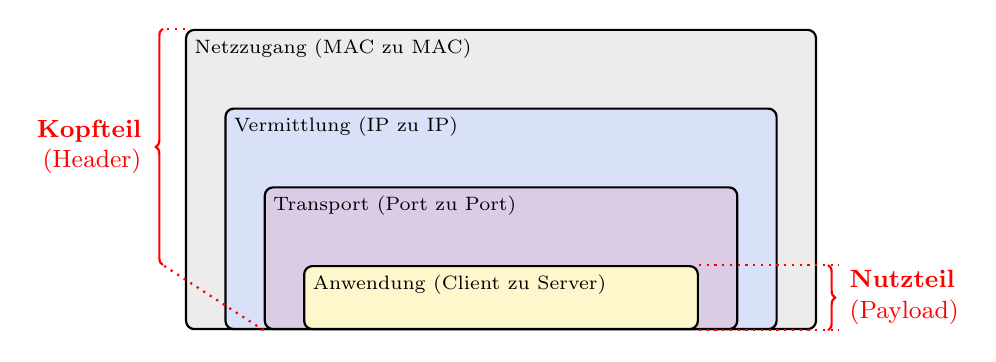
\begin{tikzpicture}[
        envelope/.style={
                draw,
                thick,
                rounded corners=3pt,
                font=\small,
                align=center
            },
        layerlabel/.style={
                font=\scriptsize,
                anchor=north west
            },
        brace/.style={decorate, decoration={brace}, red, thick},
        rbrace/.style={decorate, decoration={brace, mirror}, red, thick}
    ]

    % ---- Sizes per layer ----
    \def\increaseW{1cm}
    \def\increaseH{1cm}
    \def\moveaway{8pt}
    \def\wA{5cm}   \def\hA{.8cm}   % Anwendung
    \def\wT{\wA+\increaseW}   \def\hT{\hA+\increaseH}   % Transport
    \def\wV{\wT+\increaseW}   \def\hV{\hT+\increaseH}   % Vermittlung
    \def\wN{\wV+\increaseW}   \def\hN{\hV+\increaseH}   % Netzzugang

    % ---- Netzzugang ----
    \node[envelope, fill=dataLinkLayerColor!15, minimum width=\wN, minimum height=\hN] (net) {};
    \node[layerlabel] at (net.north west) {Netzzugang (MAC zu MAC)};

    % ---- Vermittlung ----
    \node[envelope, fill=networkLayerColor!20, minimum width=\wV, minimum height=\hV] (ver)
    at ($(net.center)+(0,-1/2*\increaseH)$) {};
    \node[layerlabel] at (ver.north west) {Vermittlung (IP zu IP)};

    % ---- Transport ----
    \node[envelope, fill=transportLayerColor!20, minimum width=\wT, minimum height=\hT] (tr)
    at ($(net.center)+(0,-2/2*\increaseH)$) {};
    \node[layerlabel] at (tr.north west) {Transport (Port zu Port)};

    % ---- Anwendung ----
    \node[envelope, fill=applicationLayerColor!20, minimum width=\wA, minimum height=\hA] (app)
    at ($(net.center)+(0,-3/2*\increaseH)$) {};
    \node[layerlabel] at (app.north west) {Anwendung (Client zu Server)};

    % ---- Braces for Header and Payload ----
    % Payload (Nutzteil): only the application data (inner payload)
    \draw[brace] ($(app.north east)+(3/2*\increaseH+4pt,0)$) -- ($(app.south east)+(3/2*\increaseH+4pt,0)$)
    node[pos=0.5, align=left, font=\small, right=4pt] {\textbf{Nutzteil}\\(Payload)};

    % dotted lines for payload
    \draw[red, dotted, thick] (app.north east) -- ($(app.north east)+(3/2*\increaseH+\moveaway,0)$);
    \draw[red, dotted, thick] (app.south east) -- ($(app.south east)+(3/2*\increaseH+\moveaway,0)$);

    % Header (Kopfteil): all headers from all layers
    \draw[rbrace] ($(net.north west)-(\moveaway,0)$) -- ($(app.north west)+(-3/2*\increaseH-\moveaway,0)$)
    node[pos=0.5, align=right, font=\small, left=4pt] {\textbf{Kopfteil}\\(Header)};

    % dotted lines for header
    \draw[red, dotted, thick] (tr.south west) -- ($(app.north west)+(-3/2*\increaseH-\moveaway,0)$);
    \draw[red, dotted, thick] (net.north west) -- ($(net.north west)-(\moveaway,0)$);
\end{tikzpicture}
\end{document}
